
\subsection{Using the Frobenius eigenvalue of $P(s)$}

\noindent
An expression which seems to be succesful for the variance is :

\centers{$ V_n =  \left( \ddot{\lambda}(-1) - { \dot{\lambda}(-1) }^2 \right) \f{n}{\ln^2 n} $}

\noindent Let's compute $\ddot{\lambda}(-1)$ with a Markov chain of order 1.

\leftcenters
    {In the paper,}
    {$ \ddot{\lambda}(-1) = \pi \ddot{P}(-1)\psi
                        + 2 \dot{\pi}(-1) \dot{P}(-1) \psi
                        - 2 \dot{\lambda}(-1) \dot{\pi}(-1) \psi $}
\noindent However, the relations defining $\pi(s)$ : 
   
        \centers{ $ \left\{
            \begin{array}{rl} \pi(s) P(s)  &= \lambda(s) \pi(s) \\
                          P(s) \psi(s) &= \lambda(s) \psi(s) \\
                          \pi(s) \psi(s) &= \lambda(s) 
            \end{array}
                    \right. $}
         
did not seem to allow me to directly compute $\dot{\pi}(s)$ (it seemed like I need
one more).
Therefore, I computed $\lambda(s)$ as the greatest 
eigenvalue of $P(s)$. Let $\chi$ the characteristic polynomial of $P(s)$,
and $\Delta$ its discrimant

\centers{$ \chi = (X - {p_{0 0}}^{-s}) 
                  (X - {p_{1 1}}^{-s}) 
                    - (p_{0 1} \, p_{1 0})^{-s} $}

\begin{egalites}
 and   & \Delta 
        & (\poo + \pii)^2 - 4[\pooii - \poiio] \\[2mm]
        && {p_{0 0}}^{-2s} 
                + {p_{1 1}}^{-s} - 2\pooii + 4\poiio
\end{egalites}

 Informally, we have this expression for $\lambda(s)$ 
where we need to decide which sign is the correct one :
\encadre{$ \lambda(s) = \f{ \poo + \pii \pm \sqrt{\Delta(s)}}{2} $}

\leftcenters
    {Since}
    {$\Delta(-1) 
        = (p_{0 0} + p_{1 1})^2 
                        - 2 p_{0 0} p_{1 1} 
                        + 4 p_{0 1} p_{1 0}
        = (p_{0 0} + p_{1 1} - 2)^2 $}
then $ \sqrt{ \Delta(-1) } = 2 - p_{0 0} - p_{1 1} = p_{0 1} + p_{1 0}$. 
Thus, picking the $+$ sign in the former expression, we verify that  
\centers{$ \lambda(-1) =  \f{ p_{0 0} + p_{1 1} + \sqrt{ \Delta(-1) } }
                                               {2} = 1 $}

\leftcenters
    {Derivating}
    {$ \dot{\lambda}(s) = \f12 \left( -\ln p_{0 0}\, \poo - \ln p_{1 1}\, \pii + \f{ \Delta'(s) }{ 2 \sqrt{\Delta(s)} } \right) $}

and the expression for $\Delta'(s)$
\centers{$ \Delta'(s) = - 2 \ln p_{0 0}\, \poodeux - 2 \ln p_{1 1}\, \piideux
                        + 2 \ln (p_{0 0} p_{1 1})\, \pooii 
                        - 4 \ln (p_{0 1} p_{1 0})\, \poiio $}
gives
\centers{$ \Delta'(-1) = - 2 \ln p_{0 0}\, {p_{0 0}}^2 - 2 \ln p_{1 1}\, {p_{1 1}}^2
                        + 2 \ln (p_{0 0} p_{1 1})\, (p_{0 0} p_{1 1})
                        - 4 \ln (p_{0 1} p_{1 0})\, (p_{0 1} p_{1 0})  $}

allowing to compute $\dot{\lambda}(-1)$. 
Numerically, we verified that $ \dot{\lambda}(-1) = h $. Derivating again yields

\centers{$ \ddot{\lambda}(s) =
                \f12 \left( \ln^2 p_{0 0} \poo + \ln^2 p_{1 1} \pii
                    + \f{ \Delta''(s) \sqrt{\Delta(s)} - \Delta'(s) \cdot \tf{\Delta'(s)}
                                                                            {2\sqrt{\Delta(s)}} }
                        {2\Delta(s)} \right)
                   $}

\leftcenters
    {with}
    {$ \Delta''(s) = 4 \ln^2 p_{0 0}\, \poodeux + 4 \ln^2 p_{1 1}\, \piideux
                     - 2 \ln^2 (p_{0 0} p_{1 1})\, \pooii
                     + 4 \ln^2 (p_{0 1} p_{1 0})\, \poiio $}

\leftencadre
    {Finally}
    {$\ddot{\lambda}(-1) = \f12 \left( \ln^2 p_{0 0}\, p_{0 0} + \ln^2 p_{1 1}\, p_{1 1}
                                + \f{ \Delta''(-1) \sqrt{\Delta(-1)} - \tf { {\Delta'(-1)}^2 }
                                                                              {2\sqrt{\Delta(-1)}} }
                                        {2\Delta(-1)} \right)
                         $}

The simulations using this coefficient for the variance are quite good. It also seems that 
this formula for the variance is equivalent to the one used in the unpublished paper 
\emph{Probabilistic Analysis of Lempel-Ziv Parsing for Markov Sources} by Leckey, 
Wormald and Neininger, but our two ways of deriving it differs. Numerical instability
might account for the tiny differences found for high $n$ values ($10^7$), although
this hasn't been verified. 

\centers{
 	 \begin{minipage}{11cm}
        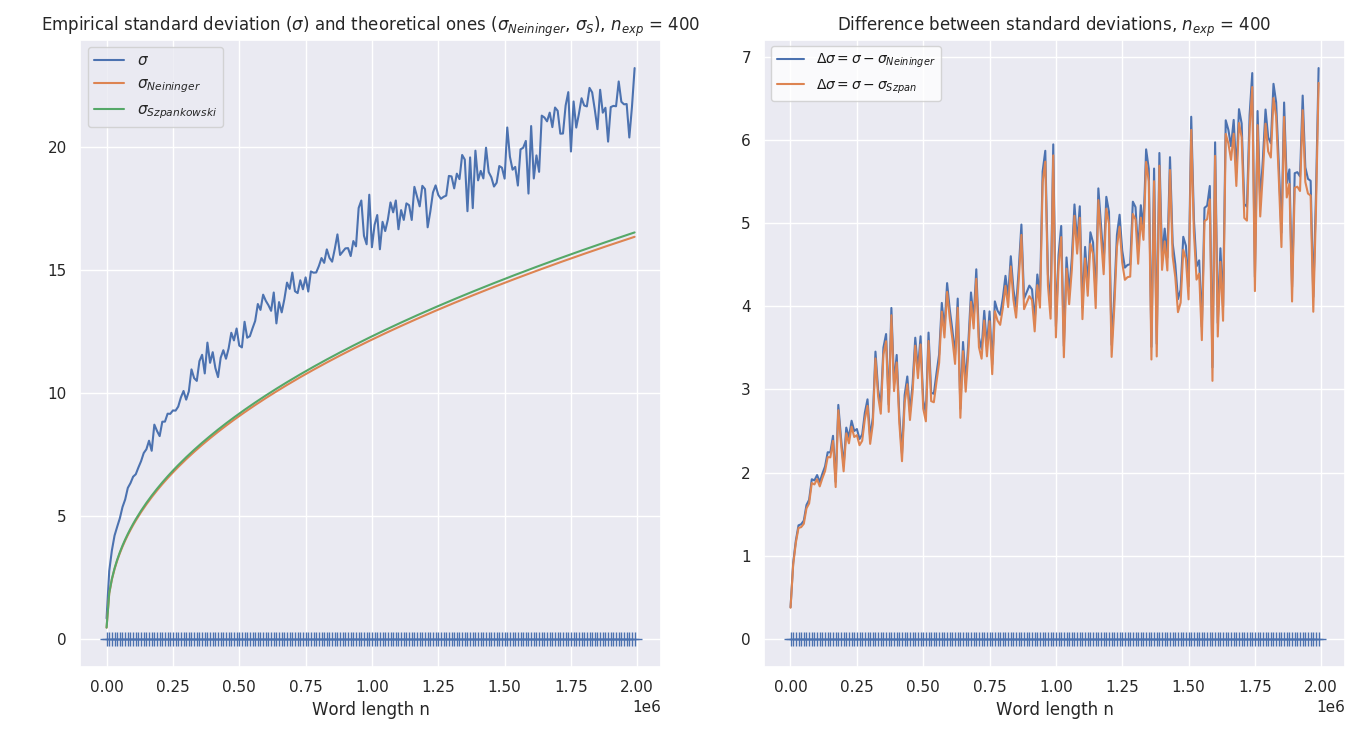
\includegraphics[width = 11cm,
        				    trim = 0 0 16.5cm 0,
        				    	clip=true]{./figs/eig_fig1.png}	
	\end{minipage} 
	}

\centers{
 	 \begin{minipage}{11cm}
        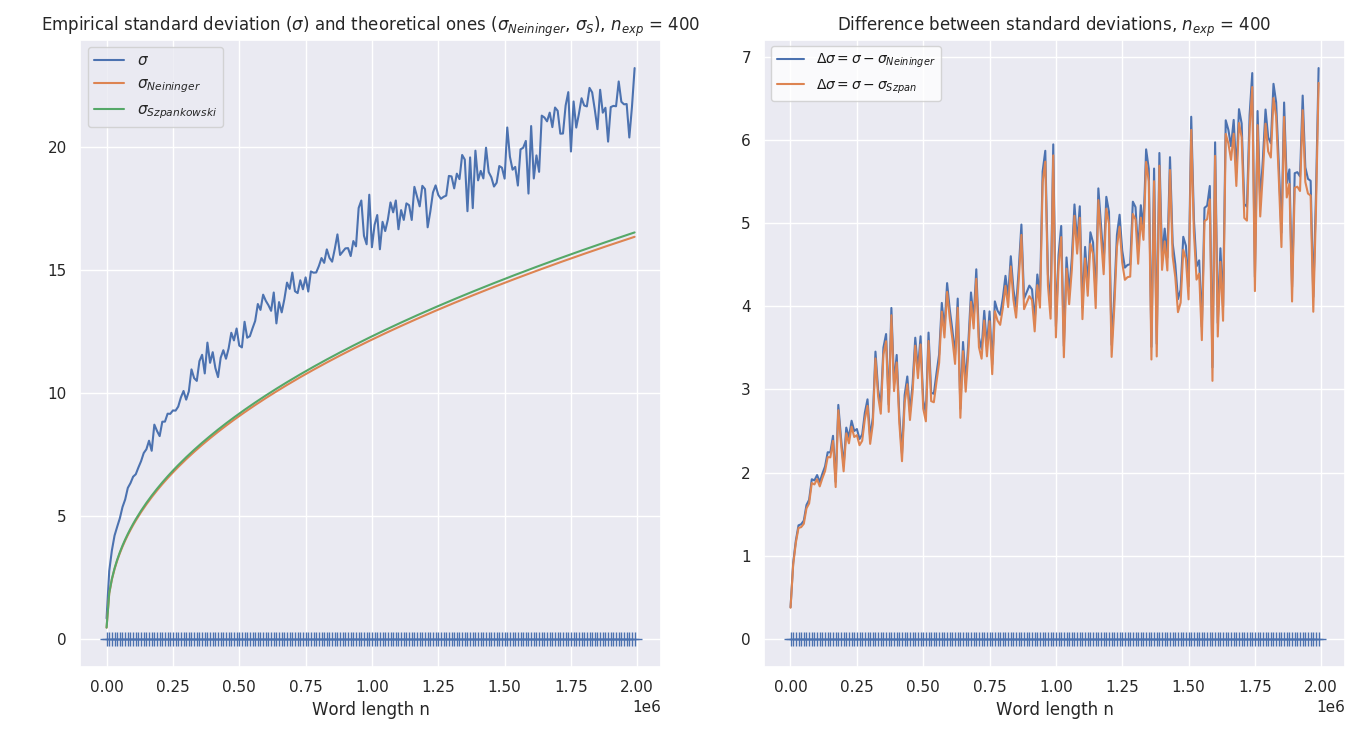
\includegraphics[width = 11cm,
        				    trim = 18.5cm 0 0 0,
        				    	clip=true]{./figs/eig_fig1.png}	
	\end{minipage} 
	}

\pagebreak
Now, for some distributions of very long words that were normalized using 
our theoretical standard deviations, and empirical means. The blue plot is 
a gaussian fit for the simulation results, which also appear as a blue histogram.
The two sets of figures are identical but obtained using different expressions.

\noindent
 	 \begin{minipage}{\textwidth}
        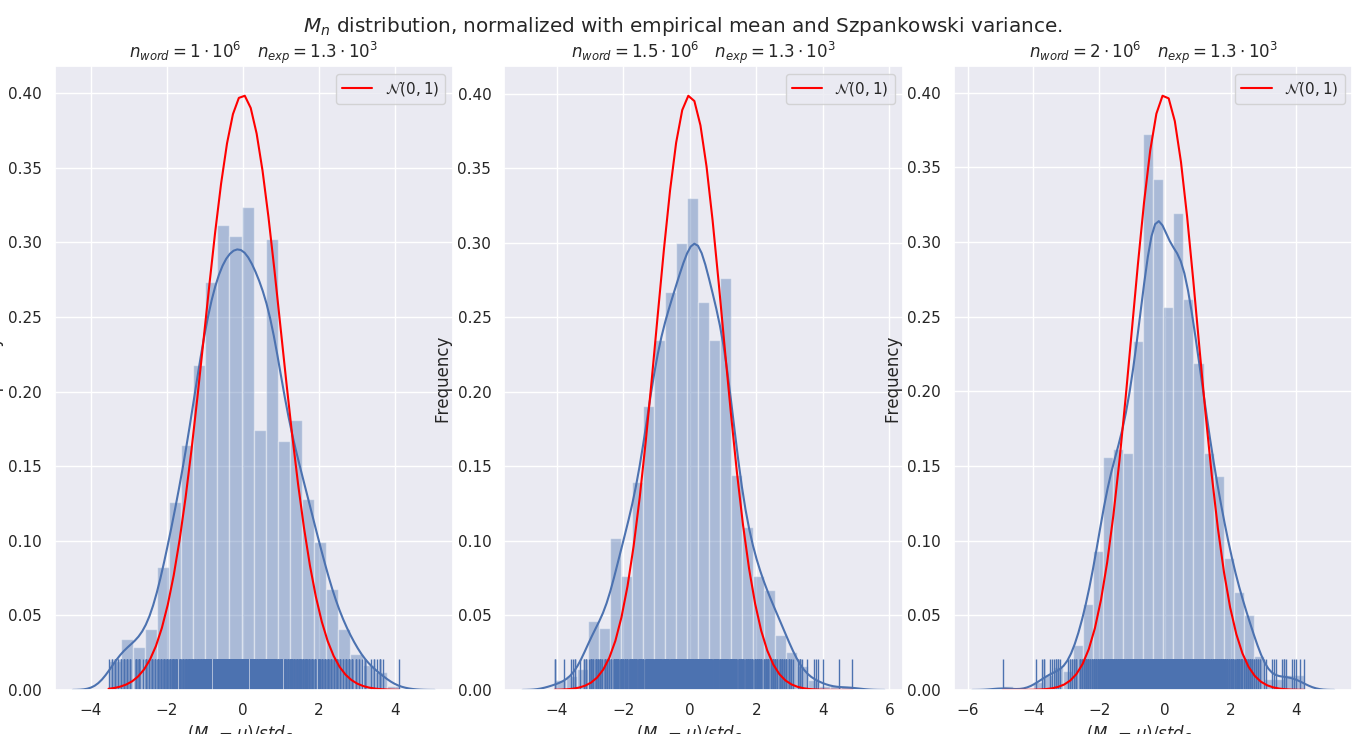
\includegraphics[width = \textwidth,
        				    trim = 0 0.5cm 0 0,
        				    	clip=true]{./figs/eig_fig2.png}	
	\end{minipage} 

\noindent
 	 \begin{minipage}{\textwidth}
        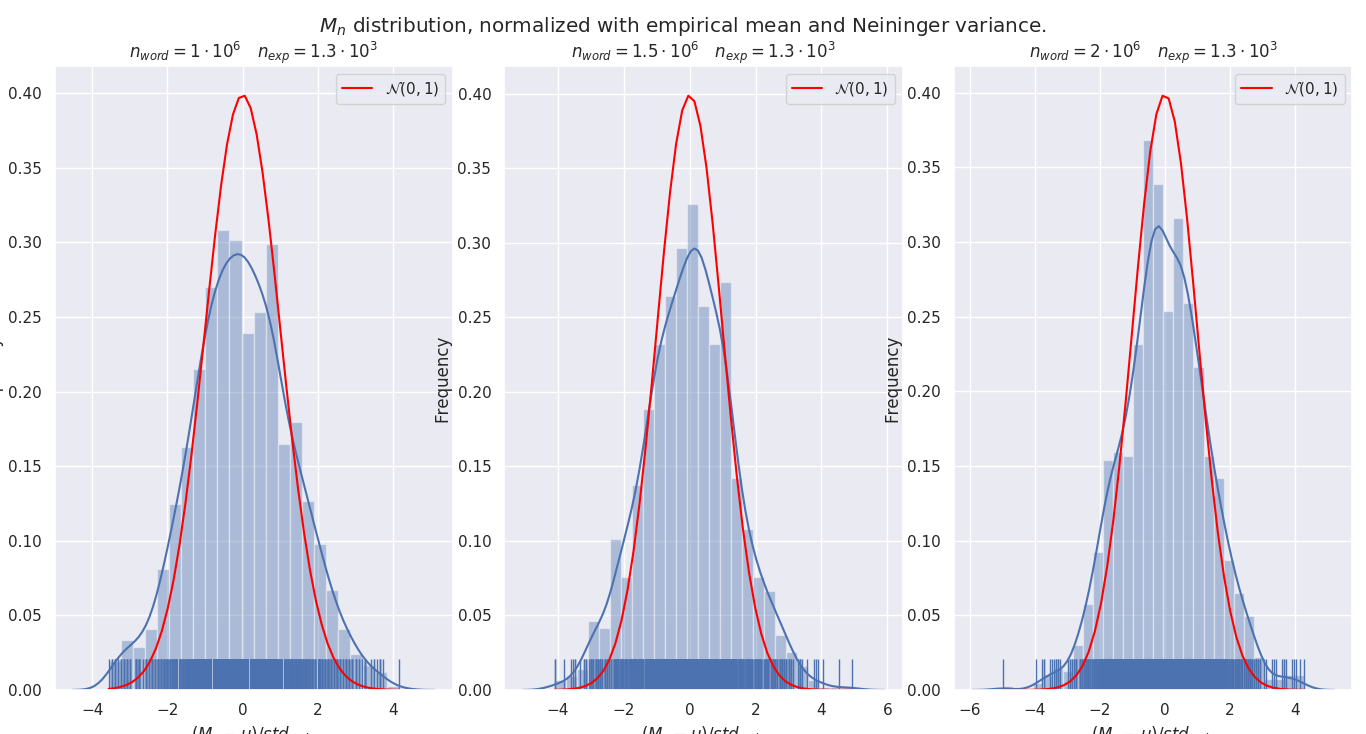
\includegraphics[width = \textwidth,
        				    trim = 0 0.5cm 0 0,
        				    	clip=true]{./figs/eig_fig3.png}	
	\end{minipage} 


\section{Conclusion}
Similar results were obtained for a variety of randomly generated Markov sources,
which seem to indicate that this formula for the variance could be proven theoretically
correct. 

\begin{remarque}
\noindent \textbf{Limits of this work}


The figures suffer from imprecision over the computation of the empirical 
variance : this is due to the difficulties encountered in computing large amounts
of long words (of size over $10^6$). The figure in appendix \ref{app:much_longer} is 
an example of this limitation : with only 100 experiments, the empirical variance 
varies a lot. Possible ideas of improvement might come from parallelization,
rewriting functions in a computationnal language such as Julia, or using/devising a datastructure
specific to the task of building very long words.

Another problem is that the space of random Markov chains (here: stochastic matrices
of size 2) is not sampled thoroughly. Sampling a small number of Markov chains uniformly
according to their entropy might be interesting as a representation of the space,
 because otherwise it would be hard to sample a large number of stochastic matrices
due to the necessity of computing large words for each of them.

Finally, the difference between empirical $V_n$ and our expression seems to be growing
very slowly with $n$. This might be a term that is negligible (\textit{i.e.} of 
order lower than $\tf{n}{\log_2^2(n)}$), or a small detail in the formula of $V_n$. 
For example, the natural base logarithm (in $\tf{n}{\ln^2(n)}$) in the eigenvalue expression works slightly
better than the one in base 2 (in $\tf{n}{\log_2^2(n)}$), with the inverse situation happening for the first 
expression ($\sigma_{\text{Neininger}}$). Anyway, the figures obtained seem to 
indicate that we are close to the exact solution.

\end{remarque}


The code for these experiments, with detailed procedures for reproducibility,
is hosted on GitHub in one of my private repositories (which I plan to make public
eventually).
Another (probably bad) way of computing $\lambda(s)$ is in appendix \ref{app:comp_lam1}. 



 
% \noindent First term is
% \centers
%     { $\pi_0 \, p_{0 0} \, \log^2 (p_{0 0}) 
%         + \pi_1 \, p_{1 0} \, \log^2 (p_{1 0}) 
%         + \pi_0 \, p_{0 1} \, \log^2 (p_{0 1}) 
%         + \pi_1 \, p_{1 1} \, \log^2 (p_{1 1})  $}

% \noindent The second is
% \centers
%     { $ - 2 \pac{
%             \dot{\pi}_0(-1) p_{0 0} \log (p_{0 0})    
%             + \dot{\pi}_1(-1) p_{1 0} \log (p_{1 0}) 
%             + \dot{\pi}_0(-1) p_{0 1} \log (p_{0 1})
%             + \dot{\pi}_1(-1) p_{1 1} \log (p_{1 1})
%         }   
%     $}

% \noindent The third is
% \centers{
%     $ - 2 \dot{\lambda}(-1) \pac{
%         \dot{\pi}_0(-1) 
%         + \dot{\pi}_1(-1)
%     }$
% }

% \noindent We 
%         have to compute $\dot{\pi}(-1)$. With 
%             $\pi(s) = (\pi_0(s), \, \pi_1(s))$, and since

% \centers{$\pi(s) P(s) = \lambda(s) \pi(s)$}

% \leftcenters
%     {then we have}
%     {$ \left\{
%         \begin{aligned}
%             {p_{0 0}}^{-s} \pi_0(s) + {p_{0 1}}^{-s} \pi_1(s) &= \lambda(s) \pi_0(s) \\
%             {p_{1 0}}^{-s} \pi_0(s) + {p_{1 1}}^{-s} \pi_1(s) &= \lambda(s) \pi_1(s) \\
%         \end{aligned}
%         \right.
%      $}

% which I'm not sure how to solve formally.
% \noindent
% solving for $\pi_0(s)$ and $\pi_1(s)$, 
% assuming $ p_{0 0} p_{1 1} \neq p_{0 1} p_{1 0} $ :

% \centers{$ \pi_0(s) = \lambda(s) \f{ \overbrace{{p_{1 1}}^{-s} - {p_{0 1}}^{-s}}^{g_0(s)} }
%                                    { \underbrace{{ (p_{0 0} p_{1 1}) }^{-s} 
%                                         - { (p_{0 1} p_{1 0}) }^{-s}}_{\delta(s)} }
%             \qquad 
%             \text{and}
%             \qquad
%        \pi_1(s) = \lambda(s) \f{ \overbrace{{p_{0 0}}^{-s} - {p_{1 0}}^{-s}}^{g_1(s)} }
%                                    { { (p_{0 0} p_{1 1}) }^{-s} 
%                                         - { (p_{0 1} p_{1 0}) }^{-s} }$}


% \leftcenters
%     {hence for $i\in\{0,1\}$}
%     {$ \dot{\pi}_i(s) = \dot{\lambda}(s) \f{g_i(s)}{\delta(s)}
%                         + \lambda(s) \f{{g_i}'(s)\delta(s) - g_i(s)\delta'(s)}
%                                         {\delta^2(s)}$}

% \leftcenters
%     {so}
%     {$ \dot{\pi}_i(-1) = h \f{g_i(-1)}{\delta(-1)}
%                         + \f{{g_i}'(-1) \delta(-1) - g_i(-1) \delta'(-1) }
%                             {\delta^2(-1)} $}

% \begin{egalites}
%     with & \delta(-1) 
%             & p_{0 0} p_{1 1} - p_{0 1} p_{1 0} \\[3mm]
%          &g_0(-1) 
%             & p_{1 1} - p_{0 1} \\[3mm]
%         &{g_0}'(-1)
%             & -\ln (p_{1 1}) p_{1 1} + \ln (p_{0 1}) p_{0 1} \\[3mm]
%         &g_1(-1)
%             & p_{0 0} - p_{1 0} \\[3mm]
%         &{g_1}'(-1) 
%             & -\ln (p_{0 0}) p_{0 0} + \ln (p_{1 0}) p_{1 0} 
% \end{egalites}


% \leftcenters
%     {where}
%     {  $\left\{
%         \begin{minipage}{0.6\textwidth}
%        $ {g_0}'(s) = - \ln(p_{1 1}) {p_{1 1}}^{-s}
%                  + \ln(p_{0 1}) {p_{0 1}}^{-s}$ \\[3mm]
%         $\delta'(s) = - \ln( p_{0 0} p_{1 1}) { (p_{0 0} p_{1 1}) }^{-s}
%                         +  \ln ( p_{0 1} p_{1 0} ) { (p_{0 1} p_{1 0}) }^{-s} $
%         \end{minipage}
%         \right.$ }



% \noindent
% Now taking $s=-1$ and re-arranging in a linear system of unknown $\dot{\pi}_0(-1)$ and $\dot{\pi}_1(-1)$ :
% \centers
%     {$ \left\{
%         \begin{aligned}
%             \dot{\pi}_0(-1) (p_{0 0} - \lambda)
%             + \dot{\pi}_1(-1) p_{0 1}
%                 &= \dot{\lambda}(-1) \pi_0
%                     +   \ln p_{0 0} \cdot p_{0 0} \pi_0
%                     +   \ln p_{0 1} \cdot p_{0 1} \pi_1 \\
%             \dot{\pi}_0(-1) p_{1 0}
%             + \dot{\pi}_1(-1) (p_{1 1} - \lambda)
%                 &= \dot{\lambda}(-1) \pi_1
%                     +  \ln p_{1 0} \cdot p_{1 0} \pi_0 
%                     +  \ln p_{1 1} \cdot p_{1 1} \pi_1
%         \end{aligned}
%         \right.
%      $}

% \noindent since
% $\dot{\lambda}(-1) = h$ and,
% $\lambda(-1) = 1$ :

% \centers
%     {$ \left\{
%         \begin{aligned}
%             \dot{\pi}_0(-1) (p_{0 0} - 1)
%             + \dot{\pi}_1(-1) p_{0 1}
%                 &= h \pi_0
%                     +   \ln p_{0 0} \cdot p_{0 0} \pi_0
%                     +   \ln p_{0 1} \cdot p_{0 1} \pi_1 \\
%             \dot{\pi}_0(-1) p_{1 0}
%             + \dot{\pi}_1(-1) (p_{1 1} - 1)
%                 &= h \pi_1
%                     +  \ln p_{1 0} \cdot p_{1 0} \pi_0 
%                     +  \ln p_{1 1} \cdot p_{1 1} \pi_1
%         \end{aligned}
%         \right.
%      $}

% \begin{egalites}
% which is  &\lambda
%         &\f{ (p_{0 0} + p_{1 1}) 
%            + \sqrt{ (p_{0 0} + p_{1 1})^2 - 4 (p_{0 0} p_{1 1} - p_{1 0} p_{0 1}) }}
%            {2}\\[3mm]
%         &&\f{ (p_{0 0} + p_{1 1}) 
%            + \sqrt{ (p_{0 0} - p_{1 1})^2 + 4 p_{1 0} p_{0 1} }}
%            {2}   
% \end{egalites}





